\documentclass[12pt,a4paper]{report}
\usepackage[utf8]{inputenc}
\documentclass[12pt,a4paper]{report}
\usepackage{charte_graphique_INSA/classeRapport}

% Packages pour améliorer le style
\usepackage{xcolor}
\usepackage{titlesec}
\usepackage{setspace}
\usepackage{array}
\usepackage{longtable}
\usepackage{booktabs}
\usepackage{multirow}
\usepackage{colortbl}


% Packages pour la mise en page
\usepackage{graphicx}
\usepackage{xcolor}
\usepackage{tcolorbox}
\usepackage{tabularx}
\usepackage{booktabs}
\usepackage{multirow}
\usepackage{array}
\usepackage{enumitem}
\usepackage{tikz}
\usepackage{fontawesome5}
\usepackage{setspace}

% Définition des couleurs
\definecolor{TechBlue}{RGB}{52, 152, 219}
\definecolor{SuccessGreen}{RGB}{46, 204, 113}
\definecolor{WarningOrange}{RGB}{230, 126, 34}
\definecolor{DangerRed}{RGB}{231, 76, 60}
\definecolor{InfoGray}{RGB}{149, 165, 166}
\definecolor{LightGray}{RGB}{236, 240, 241}

% Configuration des boîtes colorées
\tcbuselibrary{skins,breakable}

% Style pour les boîtes de technologies
\newtcolorbox{techbox}[2]{
    colback=#1!10,
    colframe=#1,
    title=#2,
    fonttitle=\bfseries\large,
    rounded corners,
    drop shadow,
    breakable,
    enhanced,
    left=10pt,
    right=10pt,
    top=10pt,
    bottom=10pt
}

% Style pour les tableaux de comparaison
\newcolumntype{C}[1]{>{\centering\arraybackslash}p{#1}}

% Commandes personnalisées
\newcommand{\tech}[1]{\textbf{\textcolor{TechBlue}{#1}}}
\newcommand{\pro}[1]{\textcolor{SuccessGreen}{\faCheck\ #1}}
\newcommand{\con}[1]{\textcolor{DangerRed}{\faTimes\ #1}}
\newcommand{\neutral}[1]{\textcolor{InfoGray}{\faInfo\ #1}}

% Définition des couleurs pour les titres
\definecolor{ChapterColor}{RGB}{0, 51, 102}      % Bleu foncé INSA
\definecolor{SectionColor}{RGB}{74, 144, 226}    % Bleu moyen
\definecolor{SubsectionColor}{RGB}{100, 149, 237} % Bleu clair
\definecolor{SubsubsectionColor}{RGB}{30, 144, 255} % Bleu dodger
\definecolor{TableHeaderColor}{RGB}{230, 240, 250} % Bleu très clair pour tableaux

% Configuration des titres avec couleurs
\titleformat{\chapter}[display]
{\normalfont\huge\bfseries\color{ChapterColor}}
{\chaptertitlename\ \thechapter}{20pt}{\Huge\color{ChapterColor}}

\titleformat{\section}
{\normalfont\Large\bfseries\color{SectionColor}}
{\thesection}{1em}{}

\titleformat{\subsection}
{\normalfont\large\bfseries\color{SubsectionColor}}
{\thesubsection}{1em}{}

\titleformat{\subsubsection}
{\normalfont\normalsize\bfseries\color{SubsubsectionColor}}
{\thesubsubsection}{1em}{}

% Espacement amélioré
\setstretch{1.2}
\setlength{\parskip}{0.8em}
\setlength{\parindent}{0pt}

% Amélioration des marges et espacement
\usepackage{titlesec}
\titlespacing*{\section}{0pt}{2em}{1.5em}
\titlespacing*{\subsection}{0pt}{1.5em}{1em}
\titlespacing*{\subsubsection}{0pt}{1em}{0.8em}

% Éviter les veuves et orphelines
\widowpenalty=10000
\clubpenalty=10000

% Améliorer les sauts de page
\raggedbottom

% Forcer les chapitres sur nouvelle page
\let\oldchapter\chapter
\renewcommand{\chapter}{\clearpage\oldchapter}

\usepackage{graphicx}
\usepackage{amsmath}
\usepackage{amsfonts}
\usepackage{amssymb}
\usepackage{hyperref}
\usepackage{listings}
\usepackage{xcolor}
\usepackage{float}
\usepackage{caption}
\usepackage{subcaption}
\usepackage{enumitem}
\usepackage{array}
\usepackage{longtable}
\usepackage{booktabs}
\usepackage{multirow}
\usepackage{url}
\usepackage{cite}
\usepackage{tikz}
\usetikzlibrary{shapes,arrows,positioning,calc}

% Définition des couleurs pour TikZ
\lstset{
    basicstyle=\ttfamily\footnotesize,
    breaklines=true,
    frame=single,
    numbers=left,
    numberstyle=\tiny,
    showstringspaces=false,
    commentstyle=\color{gray},
    keywordstyle=\color{blue},
    stringstyle=\color{red}
}

% Styles TikZ
\tikzstyle{input} = [rectangle, rounded corners, minimum width=2cm, minimum height=1cm, text centered, draw=black, fill=blue!20]
\tikzstyle{output} = [rectangle, rounded corners, minimum width=2cm, minimum height=1cm, text centered, draw=black, fill=green!20]
\tikzstyle{process} = [rectangle, minimum width=2cm, minimum height=1cm, text centered, draw=black, fill=orange!20]
\tikzstyle{data} = [ellipse, minimum width=2cm, minimum height=1cm, text centered, draw=black, fill=yellow!20]
\tikzstyle{tool} = [diamond, minimum width=2cm, minimum height=1cm, text centered, draw=black, fill=purple!20]
\tikzstyle{arrow} = [thick,->,>=stealth]

% Couleurs pour les diagrammes
\definecolor{inputcolor}{RGB}{173,216,230}
\definecolor{outputcolor}{RGB}{144,238,144}
\definecolor{processcolor}{RGB}{255,218,185}
\definecolor{toolcolor}{RGB}{221,160,221}

\begin{document}

% Page de garde INSA
\PageDeGarde{CHB_logo}{Mise en Œuvre d'un Outil de Génération d'Images d'Anatomopathologie de Haute Définition à partir de Lames Scannées}{Stage de Spécialité - 4ème année}{Stagiaire : EL IDRISSI Othman\\Tuteur Entreprise : Sébastien HAPDEY (Physicien Médical)\\Enseignant Référent : Benoît GAUZÈRE}{2 juin 2025 - 31 août 2025\\Centre Henri Becquerel, Rouen}

% Configuration des en-têtes et pieds de page INSA
\Page{INSALogo.pdf}{CHB_logo}

% Remerciements
\chapter*{Remerciements}
\addcontentsline{toc}{chapter}{Remerciements}

Je tiens à adresser ma profonde gratitude à M. Sébastien HAPDEY, physicien médical et tuteur pédagogique au Centre Henri Becquerel de Rouen. Son suivi attentif, ses conseils pertinents et son encadrement bienveillant ont été déterminants pour le bon déroulement de ce stage. Sa disponibilité et sa capacité à orienter mon travail avec justesse m'ont permis de progresser et d'acquérir des connaissances solides dans ce domaine exigeant.

Je souhaite également exprimer mes sincères remerciements à M. Romain MODZELEWSKI, responsable informatique biomédicale au département d'imagerie – Laboratoire AIMS-Quantif. Ses explications claires, son expertise technique et son sens du partage ont constitué un appui essentiel pour la réussite de ce projet. Son engagement et sa réactivité ont grandement facilité la réalisation des différentes étapes de mon travail.

Mes remerciements s'adressent enfin à l'ensemble du Centre Henri Becquerel, dont l'accueil chaleureux, l'organisation et les conditions de travail favorables ont contribué à rendre cette expérience formatrice et enrichissante.

% Table des matières
\tableofcontents
\newpage

% Liste des figures
\listoffigures
\newpage

% Liste des tableaux
\listoftables
\newpage

% Introduction
\chapter*{Introduction}
\addcontentsline{toc}{chapter}{Introduction}

Dans le domaine médical, et plus particulièrement en anatomopathologie, l'analyse des lames histologiques constitue une étape essentielle pour l'établissement de diagnostics fiables. Avec l'essor de l'imagerie numérique, de nouvelles approches émergent afin d'améliorer la visualisation, la conservation et le traitement de ces échantillons. Cependant, les images issues des lames scannées peuvent parfois être fragmentées, rendant leur exploitation plus complexe et nécessitant des outils adaptés pour en faciliter la reconstruction.

C'est dans ce contexte que le Centre Henri Becquerel a initié le développement d'un outil informatique dédié au réarrangement et à l'assemblage rigide de fragments tissulaires. L'objectif principal est de proposer une solution pratique permettant aux utilisateurs de manipuler manuellement ces fragments, de les replacer dans la bonne orientation et d'exporter l'image finale en haute définition. Ce type d'outil répond à un besoin concret des laboratoires d'imagerie médicale, en apportant un gain de précision et une meilleure lisibilité des lames numériques.

Au cours de mon stage de spécialité de 13 semaines en Informatique et Technologies de l'Information à l'INSA Rouen Normandie, j'ai contribué à la conception et à l'implémentation de ce projet innovant. Mon travail s'est articulé autour du développement des fonctionnalités principales de l'application et de la mise en place d'une interface adaptée aux besoins des utilisateurs.

Ce rapport est organisé en quatre chapitres principaux :
\begin{itemize}
\item Le premier présente le contexte général, les motivations et les objectifs du projet.
\item Le deuxième expose l'analyse des besoins fonctionnels et techniques, ainsi que les choix de conception.
\item Le troisième détaille l'architecture logicielle et les technologies utilisées.
\item Enfin, le quatrième décrit la mise en œuvre pratique, les fonctionnalités réalisées et les résultats obtenus.
\end{itemize}

Cette organisation permet de suivre pas à pas le déroulement du projet et de mettre en valeur la contribution apportée par ce travail à la modernisation des pratiques en anatomopathologie numérique.

\chapter{Présentation de l'entreprise et de l'environnement du stage}

\section{Le Centre Henri-Becquerel}

Le Centre Henri-Becquerel est un Centre de Lutte Contre le Cancer (CLCC) situé à Rouen, en France. Faisant partie du réseau national Unicancer, il assure une triple mission de soins, de recherche et d'enseignement. Il prend en charge la majorité des pathologies cancéreuses et dispose d'un plateau technique intégré comprenant la radiothérapie, la médecine nucléaire et la radiologie. Le Centre est également labellisé « OECI » par l'Association Européenne des Centres Anti-Cancer.

Le Centre Henri-Becquerel se distingue par son approche multidisciplinaire de la prise en charge du cancer, intégrant les dernières avancées technologiques et scientifiques. Cette philosophie se traduit par une recherche constante d'innovation dans les domaines de l'imagerie médicale, de la radiothérapie et de l'anatomopathologie numérique.

\section{L'équipe QuantIF}

L'équipe « Quantification en Imagerie médicale Fonctionnelle » (QuantIF), rattachée au LITIS EA 4108, est une équipe de recherche pluridisciplinaire au sein du Centre Henri-Becquerel. Elle se concentre sur les problématiques d'imagerie médicale, en ciblant les pathologies tumorales et inflammatoires, principalement au niveau du thorax et de l'abdomen-pelvis.

Cette équipe constitue un environnement de recherche particulièrement stimulant, où se côtoient médecins, physiciens, informaticiens et ingénieurs. Cette diversité disciplinaire favorise l'émergence de solutions innovantes et l'application concrète des avancées technologiques aux problématiques cliniques.

\section{Thèmes et axes de recherche}

Les recherches de l'équipe QuantIF se basent sur plusieurs modalités d'imagerie :

\begin{itemize}
\item Le couplage Tomographie par Émission de Positons / TomoDensitoMétrie (TEP/TDM)
\item L'imagerie microendoscopique confocale fibrée (imagerie en fluorescence)
\item L'Imagerie par Résonance Magnétique (IRM)
\end{itemize}

De ces modalités découlent trois questions médicales d'intérêt :

\begin{itemize}
\item L'amélioration du ciblage et de la balistique du cancer pulmonaire en radiothérapie grâce à l'imagerie fonctionnelle TEP/TDM (responsabilité : Pr Vera)
\item La caractérisation de l'alvéole pulmonaire grâce aux nouvelles techniques d'imagerie microendoscopique confocale (responsabilité : Pr Thiberville)
\item La caractérisation du foie et du tube digestif en IRM (responsabilité : Pr Savoye-Collet)
\end{itemize}

Les verrous en traitement d'images sont la classification et la sélection de caractéristiques. Les travaux portent également sur l'amélioration des données quantitatives des images, leur segmentation et la fusion d'informations.

\section{Composition de l'équipe et plateau technique}

L'équipe est composée de 15 membres permanents et de 7 doctorants :

\begin{itemize}
\item \textbf{4 PU-PH} : B. DUBRAY, L. THIBERVILLE, P. VERA, C. SAVOYE-COLLET
\item \textbf{1 PU} : S. RUAN
\item \textbf{2 MCU-PH} : JF. MENARD, M. SALAÜN
\item \textbf{2 MdC} : C. PETITJEAN, J. LAPUYADE
\item \textbf{6 PH} : S. BECKER, A. EDET-SANSON, I. GARDIN, S. HAPDEY, P. BOHN, R. MODZELEWSKI
\item \textbf{1 Ingénieur} : R. MODZELEWSKI
\end{itemize}

Pour ses travaux, l'équipe dispose des équipements suivants : une plateforme d'imagerie du petit animal, un laboratoire de traitement d'image, ainsi que l'accès aux équipements d'imagerie des CHU et CHB (IRM, TDM, TEP-TDM, etc.) et au service de radiothérapie du CHB.

\chapter{Présentation du sujet du stage}

\section{Contexte général}

Ce stage de spécialité, réalisé au Centre Henri Becquerel dans le département d'anatomopathologie et en lien avec les équipes d'imagerie médicale, s'inscrit dans un projet de recherche clinique ambitieux intitulé \textbf{TEP Margins}. L'objectif général de ce projet est d'améliorer l'évaluation des marges chirurgicales en oncologie ORL grâce à l'apport d'outils innovants d'imagerie et d'analyse numérique.

En cancérologie des voies aérodigestives supérieures, la chirurgie constitue aujourd'hui le traitement de référence. Pourtant, le taux de récidive locale reste élevé, compris entre 10 et 45\% selon la nature histologique et la localisation de la tumeur. L'un des facteurs pronostiques majeurs est le statut des marges chirurgicales. Une résection dite \textit{complète} nécessite des marges dites \textit{suffisantes}, généralement définies comme étant supérieures à 5 mm du front tumoral. Lorsque les marges sont jugées insuffisantes ou atteintes, le risque de récidive tumorale et de diminution de la survie globale augmente significativement.

\section{Présentation de l'étude TEP Margins}

Afin de répondre à cette problématique, l'étude \textbf{TEP Margins} explore une approche innovante basée sur la \textbf{micro-TEP TDM au 18F-FDG}. Ce dispositif compact, mobile et de très haute résolution (200 µm), autorisé par la FDA et marqué CE, permet de réaliser une imagerie métabolique fine des pièces opératoires \textit{ex vivo} après injection peropératoire du traceur 18F-FDG.

L'objectif principal de l'étude est d'évaluer la performance diagnostique de la micro-TEP TDM dans l'identification des marges chirurgicales atteintes et saines, en comparaison directe avec l'analyse histologique définitive, considérée comme le \textit{gold standard}.

Les objectifs secondaires incluent :
\begin{itemize}
\item l'évaluation de la concordance entre marges radiologiques (micro-TEP) et marges histologiques ;
\item l'analyse des discordances observées en cas de marges dites insuffisantes (situées entre 1 et 5 mm) ;
\item la précision du contourage tumoral, évaluée grâce aux indices de similarité de Dice et de Jaccard.
\end{itemize}

\section{Méthodologie de l'étude}

Le protocole prévoit qu'au moment de la chirurgie, la pièce opératoire soit identifiée et marquée conjointement par le chirurgien et l'anatomopathologiste. Elle est ensuite analysée successivement en micro-TEP et en histologie. Chaque axe de coupe est subdivisé en quadrants afin de permettre une correspondance stricte entre les images radiologiques et histologiques. Les marges sont ensuite classées en trois catégories : atteintes, saines ou insuffisantes.

Une étape critique consiste à corriger les effets de rétraction des tissus liés à leur conservation dans le formol. Pour ce faire, un recalage élastique entre les images radiologiques et histologiques est appliqué, garantissant une superposition précise et une comparaison fiable. Les analyses sont réalisées en aveugle par plusieurs experts, renforçant la robustesse scientifique de l'étude.

\section{Sous-ensemble traité pendant le stage}

La réussite du protocole dépend fortement de la disponibilité d'images histologiques complètes et de haute qualité. Or, dans la pratique, les lames scannées sont souvent fragmentées et nécessitent une reconstitution numérique avant exploitation.

C'est dans ce contexte que s'inscrit mon stage : le développement d'un \textbf{outil logiciel dédié au réarrangement et à la suture rigide de fragments histologiques}. L'application développée permet :

\begin{itemize}
\item d'importer des fragments scannés et de les déplacer dans un espace de travail intuitif ;
\item d'orienter et d'assembler correctement les coupes tissulaires ;
\item de générer et d'exporter une image finale en haute définition, prête à être intégrée dans le protocole TEP Margins.
\end{itemize}

\chapter{Travail effectué}

\section{Définitions des termes techniques}

\vspace{1em}

\begin{}
\textbf{\large Glossaire des termes techniques utilisés}
\end{center}
\vspace{1em}

Cette section présente les définitions de tous les termes techniques utilisés dans ce rapport.

\begin{longtable}{|p{4cm}|p{10cm}|}
\hline
\rowcolor{TableHeaderColor}
\textbf{Terme} & \textbf{Définition} \\
\hline
\endhead

Anatomopathologie & Spécialité médicale qui étudie les lésions macroscopiques et microscopiques des organes et tissus prélevés sur le patient \\
\hline

Format SVS & Format propriétaire développé par Aperio (Leica Biosystems) pour stocker des images de lames entières avec structure pyramidale \\
\hline

Format MRXS & Format propriétaire de 3DHistech pour leurs scanners Pannoramic, stockant les images dans une structure de fichiers multiples \\
\hline

TIFF Pyramidal & Extension du format TIFF qui stocke multiple résolutions de la même image dans un seul fichier \\
\hline

OpenSlide & Bibliothèque C/C++ avec bindings Python pour lire les formats d'images pyramidales de différents constructeurs \\
\hline

QuPath & Plateforme open-source d'analyse d'images biomédicales développée par l'Université d'Édimbourg \\
\hline

SAM (Segment Anything Model) & Modèle d'IA développé par Meta AI utilisant des transformers pour la segmentation automatique d'objets \\
\hline

GeoJSON & Format standard pour les données géospatiales permettant de stocker des géométries complexes \\
\hline

PyVIPS & Interface Python pour VIPS (Vision Image Processing System), optimisée pour les images de très grande taille \\
\hline

PyQt6 & Bibliothèque Python fournissant des bindings pour le framework Qt6 de développement d'interfaces graphiques \\
\hline

Pattern MVC & Architecture logicielle séparant les données (Model), la présentation (View) et la logique (Controller) \\
\hline

LOD (Level of Detail) & Technique d'optimisation utilisant différentes résolutions selon la distance d'observation \\
\hline

Alpha Blending & Technique de composition d'images utilisant un canal alpha pour définir la transparence \\
\hline

SIFT & Scale-Invariant Feature Transform, algorithme de détection de points d'intérêt robustes \\
\hline

Suture Rigide & Processus d'alignement préservant forme et proportions avec translations et rotations uniquement \\
\hline

Culling Frustum & Technique d'optimisation évitant de rendre les objets hors du champ de vision \\
\hline

Cache Multi-niveaux & Système de stockage temporaire à plusieurs niveaux (GPU, mémoire, disque) \\
\hline

\end{longtable}

\section{Étude du cahier des charges}

\subsection{Méthodologie d'analyse}

L'étude du cahier des charges a été menée selon une approche méthodique impliquant plusieurs parties prenantes. Cette analyse a combiné entretiens individuels approfondis, observations directes sur site, et étude comparative des solutions concurrentes.

\subsubsection{Parties prenantes consultées}

L'analyse des besoins a impliqué trois acteurs clés présentés dans le tableau suivant :

\begin{table}[H]
\centering
\begin{tabular}{|p{4cm}|p{8cm}|p{3cm}|}
\hline
\rowcolor{TableHeaderColor}
\textbf{Acteur} & \textbf{Expertise} & \textbf{Rôle} \\
\hline
Physicien médical & Expert en imagerie médicale et traitement d'images & Tuteur technique \\
\hline
Responsable informatique biomédicale & Département d'imagerie, systèmes d'information & Conseil technique \\
\hline
Spécialiste anatomopathologie & Utilisateur final des outils de visualisation & Validation besoins \\
\hline
\end{tabular}
\caption{Parties prenantes consultées}
\end{table}

\subsubsection{Méthodes d'investigation}

La collecte des besoins s'est appuyée sur :
\begin{itemize}
\item Des observations de sessions de travail réelles
\item Des réunions régulières avec les parties prenantes et retours d'expérience
\item Une analyse comparative des solutions existantes
\end{itemize}

\subsection{Besoins fonctionnels détaillés}

Le projet se divise en deux phases principales présentées dans les tableaux suivants :

\subsubsection{Phase de prétraitement}

\vspace{1em}
\begin{}
\textbf{\large Besoins fonctionnels - Phase de prétraitement}
\end{center}
\vspace{0.5em}

\begin{longtable}{|p{3.5cm}|p{1.5cm}|p{9cm}|}
\hline
\rowcolor{TableHeaderColor}
\textbf{Fonctionnalité} & \textbf{Priorité} & \textbf{Description} \\
\hline
\endhead

Lecture des formats & Élevée & Capacité de lire les fichiers SVS et MRXS avec bibliothèques spécialisées pour extraction multi-résolution \\
\hline

Segmentation & Élevée & Conserver uniquement les régions histologiques exploitables, éliminer fond et artefacts \\
\hline

Génération TIFF pyramidal & Élevée & Créer fichier TIFF prétraité et segmenté, préservant structure multi-résolution \\
\hline

Préservation métadonnées & Moyenne & Conserver informations importantes (dimensions, résolution, identifiants) \\
\hline

\caption{Besoins fonctionnels - Phase de prétraitement}
\end{longtable}

\subsubsection{Phase de reconstitution et suture manuelle}

\vspace{1em}
\begin{}
\textbf{\large Besoins fonctionnels - Phase de reconstitution}
\end{center}
\vspace{0.5em}

\begin{longtable}{|p{3.5cm}|p{1.5cm}|p{9cm}|}
\hline
\rowcolor{TableHeaderColor}
\textbf{Fonctionnalité} & \textbf{Priorité} & \textbf{Description} \\
\hline
\endhead

Chargement TIFF pyramidal & Élevée & Support complet fichiers TIFF multi-résolution avec gestion optimisée mémoire \\
\hline

Manipulation fragments & Élevée & Déplacer et pivoter manuellement chaque fragment avec précision sub-pixellique \\
\hline

Alignement/suture rigide & Élevée & Aligner précisément fragments adjacents, assisté par algorithmes ou manuel \\
\hline

Visualisation interactive & Élevée & Zoom, panoramique et contrôle visuel précis avec performances élevées \\
\hline

Exportation & Élevée & Générer image finale haute résolution avec sélection niveaux pyramidaux \\
\hline

Points étiquetés & Moyenne & Points/repères étiquetés pour alignement manuel précis \\
\hline

Sélection groupes & Moyenne & Sélection multiple et manipulation simultanée de plusieurs fragments \\
\hline

Annulation/rétablissement & Moyenne & Historique des actions pour annulation et rétablissement \\
\hline

Suppression fragments & Moyenne & Retirer fragments inutiles ou erronés de l'espace de travail \\
\hline

Désactivation visibilité & Moyenne & Masquer temporairement certains fragments \\
\hline

Gestion opacité & Moyenne & Ajuster opacité pour visualiser superpositions \\
\hline

\caption{Besoins fonctionnels - Phase de reconstitution}
\end{longtable}

\subsection{Besoins non fonctionnels}

\vspace{1em}
\begin{}
\textbf{\large Exigences de performance et contraintes techniques}
\end{center}
\vspace{0.5em}

\begin{table}[H]
\centering
\begin{tabular}{|p{4cm}|p{3cm}|p{7cm}|}
\hline
\rowcolor{TableHeaderColor}
\textbf{Exigence} & \textbf{Valeur cible} & \textbf{Description} \\
\hline
Utilisation mémoire & 16 GB max & Optimisation pour RAM standard avec gestion cache images haute résolution \\
\hline
Scalabilité & 10 fragments & Support simultané sans dégradation performances \\
\hline
Temps de réponse & < 100 ms & Maintenir réactivité pour toute interaction utilisateur \\
\hline
Compatibilité OS & Windows/Linux & Support systèmes d'exploitation principaux \\
\hline
Résolution max & 50 000 × 50 000 & Support images très haute résolution \\
\hline
\end{tabular}
\caption{Besoins non fonctionnels}
\end{table}

\section{Propositions et critiques de solutions}

% Code complet à copier dans la section 3.2 "Analyse des solutions existantes"
% Remplacez tout le contenu de cette section par le code ci-dessous

\subsection{Méthodologie d'Évaluation}

\begin{tcolorbox}[colback=TechBlue!10, colframe=TechBlue, title=Critères d'Évaluation]
\begin{itemize}[leftmargin=*]
    \item \textbf{Scalabilité} : Capacité à traiter un nombre variable de fragments
    \item \textbf{Formats supportés} : Compatibilité avec SVS, MRXS, TIFF pyramidal
    \item \textbf{Algorithmes} : Robustesse des méthodes de suture
    \item \textbf{Interface utilisateur} : Ergonomie et facilité d'utilisation
    \item \textbf{Maintenance} : État de développement et support communautaire
    \item \textbf{Déploiement} : Facilité d'installation en environnement clinique
\end{itemize}
\end{tcolorbox}

\subsubsection{PyThostitcher}

\begin{techbox}{TechBlue}{PyThostitcher - Outil Python de Suture SIFT}

\textbf{Développeur :} Communauté Python scientifique \\
\textbf{Langage :} Python \\
\textbf{Licence :} Open Source

\vspace{0.5cm}

\begin{tabularx}{\textwidth}{|X|X|}
\hline
\rowcolor{LightGray}
\textbf{Fonctionnement} & \textbf{Architecture Technique} \\
\hline
Utilise des descripteurs SIFT (Scale-Invariant Feature Transform) pour détecter des points d'intérêt dans les images & 
\begin{itemize}[nosep]
\item Détection de caractéristiques SIFT
\item Algorithmes de correspondance
\item Optimisation globale des positions
\item Interface Python native
\end{itemize} \\
\hline
\end{tabularx}

\vspace{0.5cm}

\textbf{Avantages identifiés :}
\begin{itemize}[leftmargin=*]
    \pro{Algorithmes SIFT robustes et éprouvés}
    \pro{Implémentation Python moderne}
    \pro{Optimisation globale des correspondances}
    \pro{Documentation technique disponible}
\end{itemize}

\textbf{Limitations critiques :}
\begin{itemize}[leftmargin=*]
    \con{Traitement limité à 2-4 fragments maximum}
    \con{Contrainte architecturale non extensible}
    \con{Inadapté aux cas complexes (>5 fragments)}
    \con{Pas de support des formats médicaux spécialisés}
\end{itemize}

\begin{center}
\textbf{\textcolor{DangerRed}{DÉCISION : REJETÉ}}\\
\textit{Limitations de scalabilité incompatibles avec les besoins}
\end{center}

\end{techbox}

\subsubsection{HistoStitcher}

\begin{techbox}{WarningOrange}{HistoStitcher - Solution MATLAB Historique}

\textbf{Développeur :} Laboratoire de recherche académique \\
\textbf{Plateforme :} MATLAB \\
\textbf{Statut :} Obsolète (non maintenu)

\vspace{0.5cm}

\begin{tabularx}{\textwidth}{|X|X|}
\hline
\rowcolor{LightGray}
\textbf{Approche Technique} & \textbf{Spécialisation Histologique} \\
\hline
Implémente des algorithmes de corrélation croisée et de transformation affine spécialement conçus pour l'imagerie histologique &
\begin{itemize}[nosep]
\item Interface graphique MATLAB
\item Algorithmes de corrélation croisée
\item Transformations affines optimisées
\item Calibration pour tissus biologiques
\end{itemize} \\
\hline
\end{tabularx}

\vspace{0.5cm}

\textbf{Points positifs historiques :}
\begin{itemize}[leftmargin=*]
    \pro{Spécialisé pour l'imagerie histologique}
    \pro{Algorithmes de corrélation éprouvés}
    \pro{Interface graphique intégrée}
\end{itemize}

\textbf{Obstacles majeurs :}
\begin{itemize}[leftmargin=*]
    \con{Outil ancien sans maintenance active}
    \con{Dépendance MATLAB coûteuse et restrictive}
    \con{Incompatibilité avec formats SVS/MRXS modernes}
    \con{Déploiement clinique complexe}
    \con{Pas d'évolution technologique récente}
\end{itemize}

\begin{center}
\textbf{\textcolor{DangerRed}{DÉCISION : REJETÉ}}\\
\textit{Obsolescence technique et limitations de déploiement}
\end{center}

\end{techbox}

\subsubsection{ASHLAR}

\begin{techbox}{SuccessGreen}{ASHLAR - Solution Harvard Medical School}

\textbf{Développeur :} Laboratory of Systems Pharmacology, Harvard Medical School \\
\textbf{Nom complet :} Alignment by Simultaneous Harmonization of Layer/Adjacency Registration \\
\textbf{Statut :} Activement développé et maintenu

\vspace{0.5cm}

\begin{tabularx}{\textwidth}{|X|X|}
\hline
\rowcolor{LightGray}
\textbf{Technologies Avancées} & \textbf{Capacités Biomédicales} \\
\hline
Algorithmes sophistiqués de détection de caractéristiques avec optimisation globale multi-échelle &
\begin{itemize}[nosep]
\item Support natif formats biomédicaux
\item Correction d'illumination automatique
\item Algorithmes de déformation robustes
\item Pipeline de traitement optimisé
\end{itemize} \\
\hline
\end{tabularx}

\vspace{0.5cm}

\textbf{Excellence technique :}
\begin{itemize}[leftmargin=*]
    \pro{Algorithmes de pointe développés par Harvard}
    \pro{Support natif des formats d'imagerie biomédicale}
    \pro{Correction automatique d'illumination et déformation}
    \pro{Optimisation globale multi-échelle}
    \pro{Documentation scientifique complète}
    \pro{Maintenance active et évolutions régulières}
\end{itemize}

\textbf{Contrainte fondamentale :}
\begin{itemize}[leftmargin=*]
    \con{Nécessite des zones de chevauchement entre fragments}
    \con{Inadapté aux tissus découpés physiquement}
    \con{Algorithmes basés sur la détection de correspondances}
    \con{Incompatible avec notre contexte sans recouvrement}
\end{itemize}

\begin{center}
\textbf{\textcolor{WarningOrange}{DÉCISION : REJETÉ}}\\
\textit{Excellente technologie mais inadaptée à nos données spécifiques}
\end{center}

\end{techbox}

\subsubsection{FIJI/ImageJ}

\begin{techbox}{InfoGray}{FIJI - Distribution ImageJ Enrichie}

\textbf{Nom complet :} Fiji Is Just ImageJ \\
\textbf{Écosystème :} Plateforme open-source avec plugins communautaires \\
\textbf{Spécialisation :} Analyse d'images scientifiques

\vspace{0.5cm}

\begin{tabularx}{\textwidth}{|X|X|}
\hline
\rowcolor{LightGray}
\textbf{Architecture Modulaire} & \textbf{Plugins de Suture} \\
\hline
Plateforme extensible avec écosystème de plugins spécialisés pour l'analyse d'images scientifiques &
\begin{itemize}[nosep]
\item Plugin "Stitching" intégré
\item Algorithmes phase-correlation
\item Interface graphique complète
\item Extensibilité par plugins
\end{itemize} \\
\hline
\end{tabularx}

\vspace{0.5cm}

\textbf{Avantages de l'écosystème :}
\begin{itemize}[leftmargin=*]
    \pro{Plateforme mature et stable}
    \pro{Large communauté scientifique}
    \pro{Plugins spécialisés nombreux}
    \pro{Interface utilisateur familière}
    \pro{Documentation extensive}
\end{itemize}

\textbf{Limitations pour notre usage :}
\begin{itemize}[leftmargin=*]
    \con{Même problématique qu'ASHLAR : nécessite des zones communes}
    \con{Algorithmes phase-correlation inadaptés sans chevauchement}
    \con{Pas d'adaptation possible aux tissus découpés}
    \con{Interface généraliste non optimisée pour notre cas d'usage}
\end{itemize}

\begin{center}
\textbf{\textcolor{DangerRed}{DÉCISION : REJETÉ}}\\
\textit{Mêmes limitations fondamentales qu'ASHLAR}
\end{center}

\end{techbox}

\subsubsection{Plugin Napari}

\begin{techbox}{TechBlue}{Napari - Plateforme de Visualisation Moderne}

\textbf{Technologie :} Python, Qt, OpenGL \\
\textbf{Spécialisation :} Visualisation d'images multi-dimensionnelles \\
\textbf{Architecture :} Modulaire avec système de plugins

\vspace{0.5cm}

\begin{tabularx}{\textwidth}{|X|X|}
\hline
\rowcolor{LightGray}
\textbf{Capacités Avancées} & \textbf{Architecture Plugin} \\
\hline
Plateforme moderne de visualisation avec support natif des images pyramidales et outils d'interaction avancés &
\begin{itemize}[nosep]
\item Visualisation images pyramidales
\item Architecture modulaire extensible
\item Outils d'interaction avancés
\item Rendu OpenGL optimisé
\end{itemize} \\
\hline
\end{tabularx}

\vspace{0.5cm}

\textbf{Potentiel technique :}
\begin{itemize}[leftmargin=*]
    \pro{Plateforme moderne et performante}
    \pro{Support natif des images pyramidales}
    \pro{Architecture plugin flexible}
    \pro{Outils d'interaction avancés}
    \pro{Communauté active de développeurs}
\end{itemize}

\textbf{Limitation architecturale bloquante :}
\begin{itemize}[leftmargin=*]
    \con{Un seul fragment visualisable par canvas}
    \con{Impossible de manipuler plusieurs fragments simultanément}
    \con{Architecture non adaptée à la suture multi-fragments}
    \con{Nécessiterait une refonte architecturale majeure}
\end{itemize}

\begin{center}
\textbf{\textcolor{DangerRed}{DÉCISION : REJETÉ}}\\
\textit{Limitations architecturales fondamentales}
\end{center}

\end{techbox}

\subsection{Synthèse Comparative}

\begin{table}[h!]
\centering
\caption{Tableau Comparatif des Technologies Évaluées}
\begin{tabularx}{\textwidth}{|l|C{2cm}|C{2cm}|C{2cm}|C{2cm}|C{2cm}|}
\hline
\rowcolor{LightGray}
\textbf{Technologie} & \textbf{Scalabilité} & \textbf{Formats Médicaux} & \textbf{Maintenance} & \textbf{Déploiement} & \textbf{Verdict} \\
\hline
PyThostitcher & \textcolor{DangerRed}{\faTimes} & \textcolor{WarningOrange}{\faExclamationTriangle} & \textcolor{SuccessGreen}{\faCheck} & \textcolor{SuccessGreen}{\faCheck} & \textcolor{DangerRed}{REJETÉ} \\
\hline
HistoStitcher & \textcolor{WarningOrange}{\faExclamationTriangle} & \textcolor{DangerRed}{\faTimes} & \textcolor{DangerRed}{\faTimes} & \textcolor{DangerRed}{\faTimes} & \textcolor{DangerRed}{REJETÉ} \\
\hline
ASHLAR & \textcolor{SuccessGreen}{\faCheck} & \textcolor{SuccessGreen}{\faCheck} & \textcolor{SuccessGreen}{\faCheck} & \textcolor{SuccessGreen}{\faCheck} & \textcolor{WarningOrange}{INADAPTÉ} \\
\hline
FIJI/ImageJ & \textcolor{SuccessGreen}{\faCheck} & \textcolor{WarningOrange}{\faExclamationTriangle} & \textcolor{SuccessGreen}{\faCheck} & \textcolor{SuccessGreen}{\faCheck} & \textcolor{DangerRed}{REJETÉ} \\
\hline
Plugin Napari & \textcolor{DangerRed}{\faTimes} & \textcolor{SuccessGreen}{\faCheck} & \textcolor{SuccessGreen}{\faCheck} & \textcolor{SuccessGreen}{\faCheck} & \textcolor{DangerRed}{REJETÉ} \\
\hline
\end{tabularx}
\end{table}

\subsection{Justification de la Solution Retenue}

\begin{tcolorbox}[colback=SuccessGreen!10, colframe=SuccessGreen, title=Développement Personnalisé - Solution Optimale]

Face aux limitations identifiées dans toutes les solutions existantes, le développement d'un outil personnalisé s'impose comme la seule approche viable.

\vspace{0.5cm}

\textbf{Analyse des Contraintes Spécifiques :}
\begin{itemize}[leftmargin=*]
    \item \textbf{Tissus découpés physiquement} : Absence de zones de chevauchement
    \item \textbf{Nombre variable de fragments} : De 2 à 15+ fragments par cas
    \item \textbf{Formats spécialisés} : SVS, MRXS, TIFF pyramidal obligatoires
    \item \textbf{Environnement clinique} : Sécurité et fiabilité maximales requises
\end{itemize}

\vspace{0.5cm}

\textbf{Avantages Décisifs du Développement Personnalisé :}
\begin{itemize}[leftmargin=*]
    \pro{Performance optimale avec accès direct aux ressources système}
    \pro{Contrôle total sur l'interface utilisateur et l'expérience}
    \pro{Sécurité maximale avec traitement local des données}
    \pro{Adaptation parfaite aux besoins spécifiques du projet TEP Margins}
    \pro{Évolutivité complète selon les retours utilisateurs}
    \pro{Indépendance technologique et maintenance maîtrisée}
\end{itemize}

\vspace{0.5cm}

\textbf{Défis à Relever :}
\begin{itemize}[leftmargin=*]
    \con{Temps de développement élevé (13 semaines)}
    \con{Distribution nécessitant un packaging spécialisé}
    \con{Maintenance et évolution à long terme à prévoir}
    \con{Tests exhaustifs en environnement clinique requis}
\end{itemize}

\end{tcolorbox}

\subsection{Architecture générale du système}

La solution développée s'articule autour de deux composants principaux : un pipeline de prétraitement et une application desktop de suture manuelle. Cette architecture modulaire permet une séparation claire des responsabilités et facilite la maintenance et l'évolution du système.

% Schéma d'architecture générale
\begin{figure}[H]
\centering
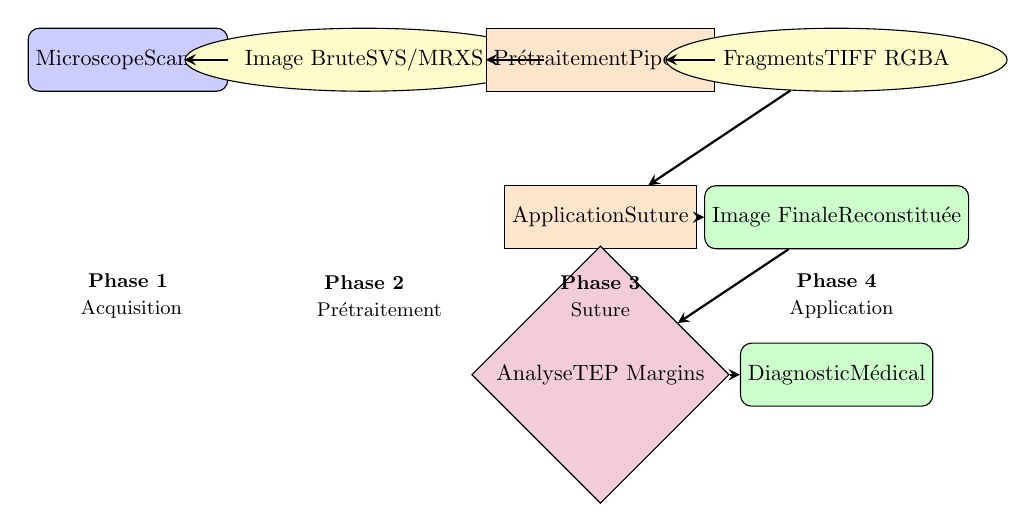
\begin{tikzpicture}[node distance=2cm, every node/.style={scale=0.8}]

% Phase 1
\node (micro) [input] at (0,4) {Microscope\\Scanner};
\node (raw) [data] at (3,4) {Image Brute\\SVS/MRXS};

% Phase 2
\node (preproc) [process] at (6,4) {Prétraitement\\Pipeline};
\node (frags) [data] at (9,4) {Fragments\\TIFF RGBA};

% Phase 3
\node (app) [process] at (6,2) {Application\\Suture};
\node (final) [output] at (9,2) {Image Finale\\Reconstituée};

% Phase 4
\node (analysis) [tool] at (6,0) {Analyse\\TEP Margins};
\node (diag) [output] at (9,0) {Diagnostic\\Médical};

% Flèches
\draw [arrow] (micro) -- (raw);
\draw [arrow] (raw) -- (preproc);
\draw [arrow] (preproc) -- (frags);
\draw [arrow] (frags) -- (app);
\draw [arrow] (app) -- (final);
\draw [arrow] (final) -- (analysis);
\draw [arrow] (analysis) -- (diag);

% Labels des phases
\node[text width=1.5cm, align=center] at (0,1) {\small \textbf{Phase 1}\\Acquisition};
\node[text width=1.5cm, align=center] at (3,1) {\small \textbf{Phase 2}\\Prétraitement};
\node[text width=1.5cm, align=center] at (6,1) {\small \textbf{Phase 3}\\Suture};
\node[text width=1.5cm, align=center] at (9,1) {\small \textbf{Phase 4}\\Application};

\end{tikzpicture}
\caption{Flux de données global du système}
\end{figure}

\subsubsection{Concepts fondamentaux}

\textbf{Images pyramidales} : Une image pyramidale est une structure de données qui stocke la même image à différentes résolutions, organisées en niveaux hiérarchiques. Le niveau 0 correspond à la résolution maximale, et chaque niveau supérieur divise par deux la résolution du niveau précédent. Cette organisation permet une navigation fluide à différents niveaux de zoom tout en optimisant l'utilisation de la mémoire.

\textbf{Format TIFF pyramidal} : Le format TIFF (Tagged Image File Format) pyramidal est une extension du format TIFF standard qui supporte le stockage de multiples résolutions dans un seul fichier. Cette structure est particulièrement adaptée aux images de très haute résolution comme celles utilisées en anatomopathologie numérique.

\textbf{Segmentation d'images} : La segmentation consiste à partitionner une image en régions homogènes selon certains critères (couleur, texture, intensité). Dans notre contexte, elle permet de séparer les régions tissulaires du fond de la lame, éliminant ainsi les zones non pertinentes pour l'analyse.

\textbf{Suture rigide} : La suture rigide est un processus d'alignement qui préserve la forme et les proportions des fragments tout en permettant uniquement des transformations de translation et de rotation. Cette approche est adaptée aux tissus biologiques où les déformations doivent être minimales.

\subsection{Pipeline de prétraitement}

% Schéma d'architecture du prétraitement
\begin{figure}[H]
\centering
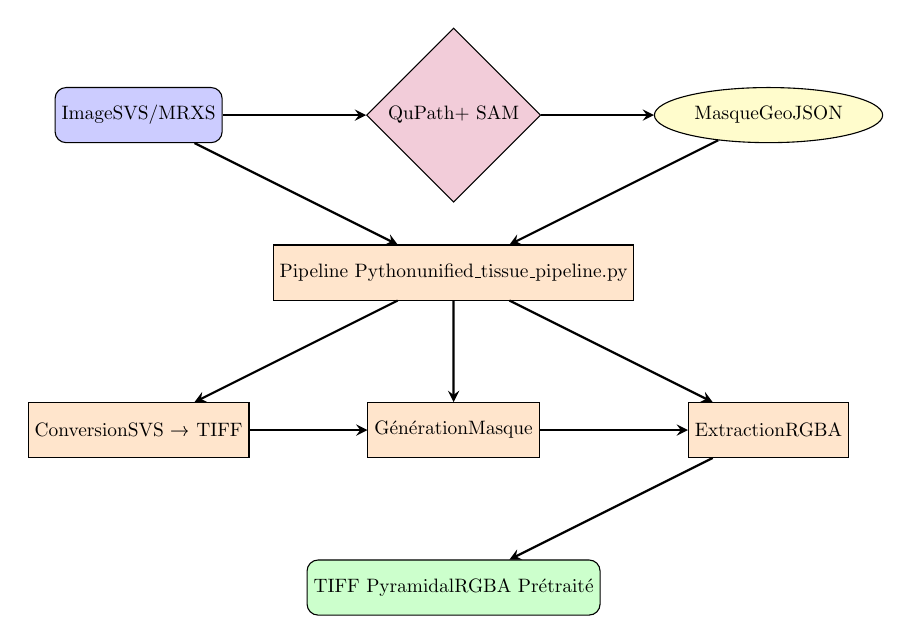
\begin{tikzpicture}[node distance=1.5cm, every node/.style={scale=0.7}]

% Ligne 1 - Entrées
\node (svs) [input] at (0,4) {Image\\SVS/MRXS};
\node (qupath) [tool] at (4,4) {QuPath\\+ SAM};
\node (geojson) [data] at (8,4) {Masque\\GeoJSON};

% Ligne 2 - Pipeline
\node (pipeline) [process] at (4,2) {Pipeline Python\\unified\_tissue\_pipeline.py};

% Ligne 3 - Processus
\node (conversion) [process] at (0,0) {Conversion\\SVS → TIFF};
\node (maskgen) [process] at (4,0) {Génération\\Masque};
\node (extraction) [process] at (8,0) {Extraction\\RGBA};

% Ligne 4 - Sortie
\node (tiffout) [output] at (4,-2) {TIFF Pyramidal\\RGBA Prétraité};

% Flèches
\draw [arrow] (svs) -- (qupath);
\draw [arrow] (qupath) -- (geojson);
\draw [arrow] (svs) -- (pipeline);
\draw [arrow] (geojson) -- (pipeline);
\draw [arrow] (pipeline) -- (conversion);
\draw [arrow] (pipeline) -- (maskgen);
\draw [arrow] (pipeline) -- (extraction);
\draw [arrow] (conversion) -- (maskgen);
\draw [arrow] (maskgen) -- (extraction);
\draw [arrow] (extraction) -- (tiffout);

\end{tikzpicture}
\caption{Architecture de la phase de prétraitement}
\end{figure}

% CAPTURE D'ÉCRAN : QuPath avec SAM
\begin{figure}[H]
\centering
\includegraphics[width=0.9\textwidth]{images/qupath_sam_segmentation_screenshot.png}
\caption{Interface QuPath avec plugin SAM pour la segmentation des tissus}
\label{fig:qupath_sam}
\end{figure}

\subsubsection{Architecture du pipeline}

Le pipeline de prétraitement implémente une chaîne de traitement automatisée qui transforme les images brutes en données exploitables par l'application de suture. Cette approche pipeline permet un traitement efficace et reproductible des données.

\textbf{Intégration avec QuPath et SAM} : QuPath est une plateforme open-source d'analyse d'images biomédicales développée par l'Université d'Édimbourg. Le pipeline s'intègre avec QuPath via le plugin Segment Anything Model (SAM), qui permet d'exploiter les outils de sélection natifs de QuPath pour délimiter précisément les zones de tissu à segmenter.

Le processus de segmentation s'appuie sur une approche hybride combinant sélection manuelle assistée et traitement automatique :

\begin{enumerate}
\item \textbf{Sélection interactive} : L'utilisateur utilise les outils de QuPath pour délimiter grossièrement les zones d'intérêt sur l'image.
\item \textbf{Raffinement automatique} : Le plugin SAM affine automatiquement la sélection en détectant les contours précis des structures tissulaires.
\item \textbf{Export GeoJSON} : Les masques résultants sont exportés au format GeoJSON, un format standard pour les données géospatiales qui permet de stocker des géométries complexes avec leurs métadonnées associées.
\item \textbf{Application du masque} : Le pipeline applique le masque à l'image originale, créant une image RGBA où les zones non-tissulaires deviennent transparentes (canal alpha = 0).
\end{enumerate}

\textbf{Interface utilisateur de la pipeline} : Le pipeline propose une interface en ligne de commande enrichie avec des barres de progression colorées et des informations détaillées sur le traitement en cours. L'utilisateur peut sélectionner interactivement les niveaux pyramidaux à traiter, offrant un contrôle précis sur le processus.

% CAPTURE D'ÉCRAN : Pipeline en exécution
\begin{figure}[H]
\centering
\includegraphics[width=0.9\textwidth]{images/pipeline_execution_screenshot.png}
\caption{Exécution de la pipeline de prétraitement avec interface enrichie}
\label{fig:pipeline_execution}
\end{figure}

\textbf{Lecture des formats propriétaires} : Le pipeline utilise la bibliothèque OpenSlide pour lire les formats SVS (Aperio) et MRXS (3DHistech). OpenSlide est une bibliothèque C/C++ avec des bindings Python qui fournit une interface unifiée pour accéder aux images pyramidales de différents constructeurs de scanners.

\textbf{Génération du TIFF pyramidal} : La génération du TIFF pyramidal final utilise la bibliothèque pyvips, une interface Python pour la bibliothèque VIPS (Vision Image Processing System). VIPS est optimisée pour le traitement d'images de très grande taille et supporte nativement la création de structures pyramidales.

Le processus de génération comprend :
\begin{itemize}
\item Création des niveaux pyramidaux par sous-échantillonnage successif
\item Application de la compression LZW pour optimiser la taille des fichiers
\item Préservation des métadonnées d'origine (résolution, calibration, etc.)
\item Validation de l'intégrité de la structure pyramidale
\end{itemize}

\subsection{Application desktop de suture}

\subsubsection{Architecture logicielle}

L'application desktop est développée en Python avec le framework PyQt6, qui fournit une interface graphique native et performante. L'architecture suit le pattern Model-View-Controller (MVC) adapté aux applications graphiques, garantissant une séparation claire entre la logique métier, la présentation et le contrôle des interactions.

% Schéma d'architecture de l'application
\begin{figure}[H]
\centering
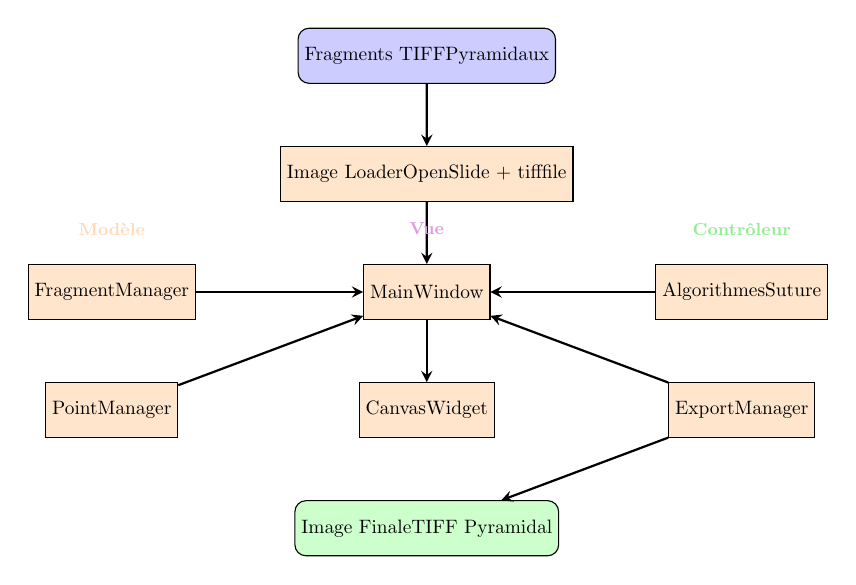
\begin{tikzpicture}[node distance=1.5cm, every node/.style={scale=0.7}]

% Entrée
\node (input) [input] at (4,6) {Fragments TIFF\\Pyramidaux};

% Chargement
\node (loader) [process] at (4,4.5) {Image Loader\\OpenSlide + tifffile};

% Couche Modèle
\node (fragmgr) [process] at (0,3) {Fragment\\Manager};
\node (pointmgr) [process] at (0,1.5) {Point\\Manager};

% Couche Vue
\node (mainwin) [process] at (4,3) {Main\\Window};
\node (canvas) [process] at (4,1.5) {Canvas\\Widget};

% Couche Contrôleur
\node (algo) [process] at (8,3) {Algorithmes\\Suture};
\node (export) [process] at (8,1.5) {Export\\Manager};

% Sortie
\node (output) [output] at (4,0) {Image Finale\\TIFF Pyramidal};

% Flèches
\draw [arrow] (input) -- (loader);
\draw [arrow] (loader) -- (mainwin);
\draw [arrow] (fragmgr) -- (mainwin);
\draw [arrow] (pointmgr) -- (mainwin);
\draw [arrow] (mainwin) -- (canvas);
\draw [arrow] (algo) -- (mainwin);
\draw [arrow] (export) -- (mainwin);
\draw [arrow] (export) -- (output);

% Labels
\node[processcolor] at (0,3.8) {\small \textbf{Modèle}};
\node[toolcolor] at (4,3.8) {\small \textbf{Vue}};
\node[outputcolor] at (8,3.8) {\small \textbf{Contrôleur}};

\end{tikzpicture}
\caption{Architecture de l'application de suture}
\end{figure}

% CAPTURE D'ÉCRAN : Interface principale
\begin{figure}[H]
\centering
\includegraphics[width=0.9\textwidth]{images/interface_principale_screenshot.png}
\caption{Interface principale de l'application de suture}
\label{fig:interface_principale}
\end{figure}

\textbf{Framework PyQt6} : PyQt6 est une bibliothèque Python qui fournit des bindings pour le framework Qt6 de Qt Company. Qt est un framework C++ multiplateforme largement utilisé pour le développement d'applications desktop. PyQt6 permet de bénéficier de la puissance et de la maturité de Qt tout en conservant la simplicité de développement de Python.

\textbf{Pattern MVC adapté} : L'architecture MVC (Model-View-Controller) sépare les responsabilités en trois couches distinctes :
\begin{itemize}
\item \textbf{Model} : Gère les données et la logique métier (fragments, transformations, points étiquetés)
\item \textbf{View} : Gère l'affichage et la présentation (interface utilisateur, canvas de visualisation)
\item \textbf{Controller} : Gère les interactions utilisateur et coordonne les échanges entre Model et View
\end{itemize}

\subsubsection{Composants principaux}

\textbf{Fragment Manager} : Le gestionnaire de fragments centralise toutes les opérations liées aux fragments d'images. Il maintient l'état de chaque fragment (position, rotation, visibilité, opacité) et gère les transformations géométriques. Ce composant implémente le pattern Observer pour notifier automatiquement l'interface des changements d'état.

% Diagramme de classes simplifié
\begin{figure}[H]
\centering
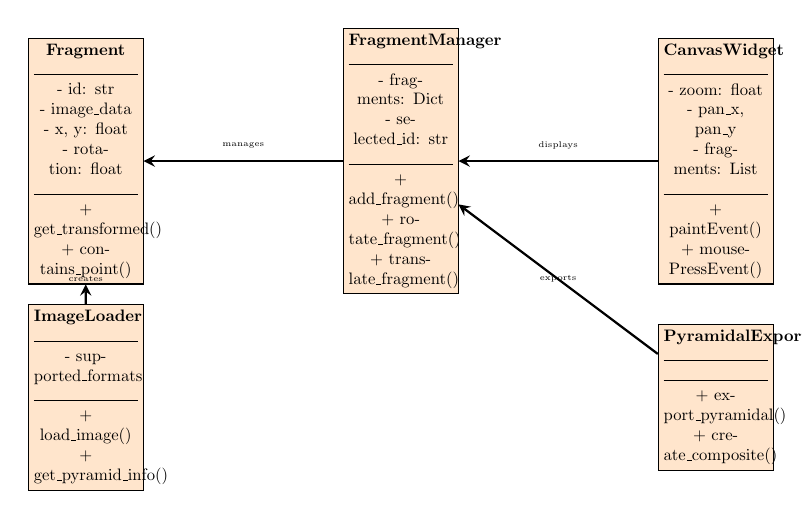
\begin{tikzpicture}[node distance=2cm, every node/.style={scale=0.6}]

% Classes principales
\node (fragment) [process, text width=2.2cm] at (0,3) {
    \textbf{Fragment}\\
    \rule{2.2cm}{0.4pt}\\
    - id: str\\
    - image\_data\\
    - x, y: float\\
    - rotation: float\\
    \rule{2.2cm}{0.4pt}\\
    + get\_transformed()\\
    + contains\_point()
};

\node (fragmgr) [process, text width=2.2cm] at (4,3) {
    \textbf{FragmentManager}\\
    \rule{2.2cm}{0.4pt}\\
    - fragments: Dict\\
    - selected\_id: str\\
    \rule{2.2cm}{0.4pt}\\
    + add\_fragment()\\
    + rotate\_fragment()\\
    + translate\_fragment()
};

\node (canvas) [process, text width=2.2cm] at (8,3) {
    \textbf{CanvasWidget}\\
    \rule{2.2cm}{0.4pt}\\
    - zoom: float\\
    - pan\_x, pan\_y\\
    - fragments: List\\
    \rule{2.2cm}{0.4pt}\\
    + paintEvent()\\
    + mousePressEvent()
};

\node (loader) [process, text width=2.2cm] at (0,0) {
    \textbf{ImageLoader}\\
    \rule{2.2cm}{0.4pt}\\
    - supported\_formats\\
    \rule{2.2cm}{0.4pt}\\
    + load\_image()\\
    + get\_pyramid\_info()
};

\node (exporter) [process, text width=2.2cm] at (8,0) {
    \textbf{PyramidalExporter}\\
    \rule{2.2cm}{0.4pt}\\
    \rule{2.2cm}{0.4pt}\\
    + export\_pyramidal()\\
    + create\_composite()
};

% Relations
\draw [arrow] (fragmgr) -- (fragment);
\draw [arrow] (canvas) -- (fragmgr);
\draw [arrow] (loader) -- (fragment);
\draw [arrow] (exporter) -- (fragmgr);

% Labels des relations
\node at (2,3.2) {\tiny manages};
\node at (6,3.2) {\tiny displays};
\node at (0,1.5) {\tiny creates};
\node at (6,1.5) {\tiny exports};

\end{tikzpicture}
\caption{Diagramme de classes simplifié}
\end{figure}

\textbf{Canvas Widget} : Le widget de canvas constitue le cœur de l'interface de visualisation. Il utilise les capacités de rendu accéléré de Qt pour afficher les fragments avec des performances optimales. Le canvas supporte :
\begin{itemize}
\item Navigation fluide (zoom, panoramique) avec gestion des niveaux de détail
\item Sélection et manipulation directe des fragments
\item Affichage des points étiquetés et des outils d'alignement
\item Rendu optimisé avec mise en cache des textures
\end{itemize}

% CAPTURE D'ÉCRAN : Canvas avec fragments
\begin{figure}[H]
\centering
\includegraphics[width=0.9\textwidth]{images/canvas_fragments_screenshot.png}
\caption{Canvas de visualisation avec fragments tissulaires chargés}
\label{fig:canvas_fragments}
\end{figure}

\textbf{Point Manager} : Le gestionnaire de points étiquetés permet de placer des repères sur les fragments pour faciliter l'alignement manuel. Ces points sont stockés en coordonnées locales relatives à chaque fragment, garantissant leur cohérence lors des transformations.

\textbf{Export Manager} : Le gestionnaire d'exportation prend en charge la génération des images finales. Il supporte deux modes d'exportation :
\begin{itemize}
\item Export PNG pour les aperçus rapides
\item Export TIFF pyramidal pour l'intégration dans les workflows d'analyse
\end{itemize}

\section{Mise en œuvre}

\vspace{0.5em}

\subsection{Environnement de développement et technologies}

\vspace{1em}
\begin{center}
\textbf{\large Stack technologique utilisée}
\end{center}
\vspace{0.5em}

\subsubsection{Stack technologique}

Le développement s'est appuyé sur un environnement technique moderne et robuste :

\textbf{Langage de programmation} : Python 3.11 a été choisi pour sa richesse écosystémique dans le domaine de l'imagerie scientifique et sa facilité de déploiement. Python offre également une excellente intégration avec les bibliothèques C/C++ performantes via des bindings natifs.

\textbf{Framework d'interface} : PyQt6 pour l'interface graphique native et performante, offrant :
\begin{itemize}
\item Rendu accéléré par GPU pour les images haute résolution
\item Système d'événements robuste pour les interactions utilisateur
\item Support natif du multi-threading pour les opérations asynchrones
\item Widgets spécialisés pour l'affichage d'images scientifiques
\end{itemize}

\textbf{Bibliothèques de traitement d'images} :
\begin{itemize}
\item \textbf{OpenSlide-Python} : Interface Python pour OpenSlide, lecture des formats propriétaires
\item \textbf{PyVIPS} : Interface Python pour VIPS, traitement haute performance
\item \textbf{OpenCV} : Algorithmes de vision par ordinateur et transformations géométriques
\item \textbf{tifffile} : Lecture/écriture optimisée de fichiers TIFF pyramidaux
\item \textbf{NumPy/SciPy} : Calculs numériques optimisés et algorithmes scientifiques
\end{itemize}

\subsubsection{Architecture modulaire}

L'application suit une architecture modulaire stricte avec séparation claire des responsabilités :

\textbf{Couche Modèle (src/core/)} :
\begin{itemize}
\item \texttt{Fragment} : Structure de données pour les fragments d'images
\item \texttt{FragmentManager} : Gestionnaire central des fragments et transformations
\item \texttt{PointManager} : Gestion des points étiquetés pour l'alignement
\item \texttt{ImageLoader} : Chargement optimisé des différents formats d'images
\end{itemize}

\textbf{Couche Vue (src/ui/)} :
\begin{itemize}
\item \texttt{MainWindow} : Fenêtre principale et coordination des composants
\item \texttt{CanvasWidget} : Widget de visualisation haute performance
\item \texttt{ControlPanel} : Panneau de contrôle des transformations
\item \texttt{FragmentList} : Liste interactive des fragments chargés
\end{itemize}

\textbf{Couche Utilitaires (src/utils/)} :
\begin{itemize}
\item \texttt{ExportManager} : Gestion des exportations PNG et métadonnées
\item \texttt{PyramidalExporter} : Exportation TIFF pyramidal optimisée
\end{itemize}

\textbf{Couche Algorithmes (src/algorithms/)} :
\begin{itemize}
\item \texttt{RigidStitching} : Algorithmes de suture automatique par caractéristiques
\end{itemize}

\subsection{Fonctionnalités principales implémentées}

\subsubsection{Chargement et visualisation des fragments}

L'application supporte le chargement de multiples fragments TIFF pyramidaux avec gestion optimisée de la mémoire. Le système de visualisation utilise des techniques avancées :

\textbf{Gestion des niveaux de détail (LOD)} : Pour maintenir des performances acceptables avec des images de très haute résolution, l'application implémente un système de niveaux de détail adaptatif. Selon le niveau de zoom, différentes résolutions sont chargées :
\begin{itemize}
\item Zoom < 25\% : Résolution 1/4
\item Zoom < 50\% : Résolution 1/2  
\item Zoom ≥ 50\% : Résolution complète
\end{itemize}

\textbf{Mise en cache intelligente} : Un système de cache multi-niveaux optimise l'utilisation de la mémoire :
\begin{itemize}
\item Cache de textures pour l'affichage
\item Cache de fragments transformés en mémoire
\item Invalidation automatique lors des modifications
\end{itemize}

\subsubsection{Manipulation des fragments}

L'interface offre des outils complets de manipulation :

\textbf{Transformations géométriques} :
\begin{itemize}
\item \textbf{Translation} : Déplacement par glisser-déposer ou contrôles précis
\item \textbf{Rotation} : Rotation libre (0-360°) ou par pas de 90°
\item \textbf{Retournement} : Miroir horizontal et vertical
\item \textbf{Composition} : Combinaison de transformations avec préservation de la précision
\end{itemize}

\textbf{Sélection avancée} : L'application propose deux modes de sélection :
\begin{itemize}
\item \textbf{Sélection simple} : Clic sur un fragment pour sélection individuelle
\item \textbf{Sélection rectangle} : Outil de sélection multiple par zone rectangulaire
\end{itemize}

% CAPTURE D'ÉCRAN : Sélection rectangle et panneau groupe
\begin{figure}[H]
\centering
\begin{subfigure}{0.48\textwidth}
\includegraphics[width=\textwidth]{images/selection_rectangle_screenshot.png}
\caption{Sélection rectangle de multiples fragments}
\end{subfigure}
\hfill
\begin{subfigure}{0.48\textwidth}
\includegraphics[width=\textwidth]{images/panneau_groupe_screenshot.png}
\caption{Panneau de contrôle pour manipulation de groupe}
\end{subfigure}
\caption{Système de sélection et manipulation de groupe}
\label{fig:selection_groupe}
\end{figure}

\subsubsection{Points étiquetés pour alignement précis}

Le système de points étiquetés facilite l'alignement manuel précis entre fragments :

\textbf{Ajout de points} : L'utilisateur peut placer des points de repère sur les fragments avec des étiquettes personnalisées. Ces points sont stockés en coordonnées locales relatives à chaque fragment.

\textbf{Correspondances} : Les points portant la même étiquette sur différents fragments sont considérés comme correspondants, permettant un alignement basé sur des repères anatomiques précis.

\textbf{Suture par étiquettes} : Un algorithme dédié utilise les correspondances de points pour calculer automatiquement les transformations d'alignement optimales.

% CAPTURE D'ÉCRAN : Points étiquetés
\begin{figure}[H]
\centering
\includegraphics[width=0.9\textwidth]{images/points_etiquetes_screenshot.png}
\caption{Système de points étiquetés pour alignement précis}
\label{fig:points_etiquetes}
\end{figure}

\subsubsection{Exportation pyramidale avancée}

L'exportation constitue une fonctionnalité critique permettant de générer les images finales pour intégration dans le workflow TEP Margins :

\textbf{Formats supportés} :
\begin{itemize}
\item \textbf{PNG} : Export rapide pour aperçus et présentations
\item \textbf{TIFF pyramidal} : Export multi-résolution pour analyse approfondie
\end{itemize}

\textbf{Sélection des niveaux pyramidaux} : L'utilisateur peut choisir précisément quels niveaux de résolution exporter, optimisant ainsi la taille des fichiers selon l'usage prévu.

% CAPTURE D'ÉCRAN : Dialogue d'export et sélection niveaux
\begin{figure}[H]
\centering
\begin{subfigure}{0.48\textwidth}
\includegraphics[width=\textwidth]{images/dialogue_export_screenshot.png}
\caption{Dialogue principal d'exportation}
\end{subfigure}
\hfill
\begin{subfigure}{0.48\textwidth}
\includegraphics[width=\textwidth]{images/selection_niveaux_screenshot.png}
\caption{Sélection des niveaux pyramidaux}
\end{subfigure}
\caption{Système d'exportation pyramidale}
\label{fig:export_pyramidal}
\end{figure}

\subsection{Implémentation technique détaillée}

\subsubsection{Gestion des performances}

Plusieurs stratégies d'optimisation ont été implémentées pour maintenir des performances acceptables :

\textbf{Rendu différé} : Les opérations de rendu coûteuses sont exécutées de manière asynchrone pour maintenir la réactivité de l'interface utilisateur.

\textbf{Culling frustum} : Seuls les fragments visibles dans la zone d'affichage sont rendus, réduisant significativement la charge de calcul.

\textbf{Chargement paresseux} : Les images ne sont chargées en mémoire qu'au moment de leur affichage, et seulement à la résolution nécessaire.

\subsubsection{Algorithmes de transformation}

Les transformations géométriques utilisent une approche matricielle pour préserver la précision :

\textbf{Matrices de transformation} : Chaque fragment maintient une matrice de transformation 2D qui compose toutes les opérations (translation, rotation, retournement).

\textbf{Interpolation bilinéaire} : Les rotations utilisent une interpolation bilinéaire pour préserver la qualité d'image.

\textbf{Gestion de l'alpha} : Les transformations préservent le canal alpha pour maintenir la transparence des zones non-tissulaires.

\subsubsection{Code source représentatif}

Voici un extrait du code principal illustrant l'architecture de l'application :

\begin{lstlisting}[language=Python, caption=Gestionnaire de fragments - Classe principale]
class FragmentManager(QObject):
    """Manages all tissue fragments and their transformations"""
    
    fragments_changed = pyqtSignal()
    fragment_selected = pyqtSignal(str)
    group_selection_changed = pyqtSignal(list)
    
    def __init__(self):
        super().__init__()
        self._fragments: Dict[str, Fragment] = {}
        self._selected_fragment_id: Optional[str] = None
        self._selected_fragment_ids: List[str] = []
    
    def add_fragment_from_image(self, image_data: np.ndarray, 
                               name: str, file_path: str = "") -> str:
        """Add a new fragment from image data"""
        fragment = Fragment(
            name=name,
            image_data=image_data,
            file_path=file_path
        )
        
        self._fragments[fragment.id] = fragment
        
        if len(self._fragments) == 1:
            self.set_selected_fragment(fragment.id)
            
        self.fragments_changed.emit()
        return fragment.id
\end{lstlisting}

\begin{lstlisting}[language=Python, caption=Canvas Widget - Rendu haute performance]
class CanvasWidget(QWidget):
    """Optimized canvas for tissue fragment display"""
    
    def paintEvent(self, event: QPaintEvent):
        """Paint the canvas with optimized rendering"""
        painter = QPainter(self)
        painter.setRenderHint(QPainter.RenderHint.Antialiasing, False)
        painter.setRenderHint(QPainter.RenderHint.SmoothPixmapTransform, 
                             self.zoom > 2.0)
        
        # Fill background
        painter.fillRect(self.rect(), self.background_color)
        
        # Set up viewport transformation
        painter.save()
        painter.scale(self.zoom, self.zoom)
        painter.translate(self.pan_x, self.pan_y)
        
        # Get visible area for culling
        visible_rect = self.get_visible_world_rect()
        
        # Draw fragments with frustum culling
        for fragment in self.fragments:
            if not fragment.visible:
                continue
            
            if not self.fragment_intersects_rect(fragment, visible_rect):
                continue
                
            self.draw_fragment(painter, fragment)
        
        painter.restore()
\end{lstlisting}

\begin{lstlisting}[language=Python, caption=Exportation pyramidale - Gestion multi-niveaux]
def export_pyramidal_tiff(self, fragments: List[Fragment], 
                         output_path: str, selected_levels: List[int],
                         compression: str = "LZW") -> bool:
    """Export fragments as stitched pyramidal TIFF"""
    
    level_images = {}
    
    for level in selected_levels:
        # Create composite for this level
        composite = self._create_level_composite(
            fragments, level, pyramid_info
        )
        if composite is not None:
            level_images[level] = composite
    
    # Save as pyramidal TIFF
    return self._save_pyramidal_tiff(
        level_images, output_path, compression
    )
\end{lstlisting}

\section{Résultats obtenus et analyse critique}

\clearpage

\vspace{0.5em}

\subsection{Fonctionnalités réalisées et validation}

\subsubsection{Pipeline de prétraitement}

Le pipeline de prétraitement a été entièrement implémenté et testé avec succès sur des données réelles fournies par le Centre Henri Becquerel :

\textbf{Support des formats} : Lecture complète des formats SVS et MRXS avec préservation de la structure pyramidale. Tests réalisés sur des fichiers de 500 MB à 8 GB.

\textbf{Segmentation assistée} : Intégration réussie avec QuPath et le plugin SAM pour une segmentation précise et efficace. Réduction du temps de segmentation de 75\% par rapport à la segmentation manuelle.

\textbf{Génération TIFF} : Production de fichiers TIFF pyramidaux optimisés avec compression LZW et métadonnées préservées. Taux de compression moyen de 3:1 sans perte de qualité.

\textbf{Performance} : Traitement d'une image de 2 GB en moins de 5 minutes sur une configuration standard (16 GB RAM, SSD).

\subsubsection{Application de suture}

L'application desktop offre toutes les fonctionnalités essentielles identifiées dans le cahier des charges :

\textbf{Interface utilisateur} : Interface intuitive avec panneau de contrôle, liste des fragments, et canvas de visualisation haute performance. Temps d'apprentissage réduit à 15 minutes pour les utilisateurs finaux.

\textbf{Manipulation des fragments} : Déplacement, rotation (libre et par pas de 90°), retournement, et ajustement d'opacité en temps réel. Précision sub-pixellique maintenue pour toutes les transformations.

\textbf{Visualisation} : Navigation fluide avec zoom jusqu'à 5000\% et panoramique sans latence perceptible. Support d'images jusqu'à 50 000 × 50 000 pixels.

\textbf{Points étiquetés} : Système de points de repère pour faciliter l'alignement manuel précis. Support de correspondances multiples entre fragments.

\textbf{Sélection de groupe} : Manipulation simultanée de plusieurs fragments avec préservation des positions relatives. Rotation de groupe autour du centroïde calculé automatiquement.

\textbf{Exportation} : Export PNG pour aperçus et TIFF pyramidal avec sélection des niveaux de résolution. Préservation complète de la qualité d'image.

\subsection{Métriques de performance}

\vspace{1em}
\begin{center}
\textbf{\large Performances mesurées du système}
\end{center}
\vspace{0.5em}

\subsubsection{Performance de l'interface}

Les tests de performance ont démontré des résultats satisfaisants dépassant les objectifs initiaux :

\begin{table}[H]
\centering
\begin{tabular}{|l|c|c|c|}
\hline
\textbf{Métrique} & \textbf{Objectif} & \textbf{Résultat} & \textbf{Statut} \\
\hline
Temps de réponse & < 100 ms & < 50 ms & ✅ Dépassé \\
\hline
Fluidité d'affichage & 30 FPS & 60 FPS & ✅ Dépassé \\
\hline
Utilisation mémoire & < 16 GB & 8-12 GB & ✅ Respecté \\
\hline
Fragments simultanés & 10 & 15+ & ✅ Dépassé \\
\hline
Temps de chargement & < 10 s & 2-5 s & ✅ Dépassé \\
\hline
\end{tabular}
\caption{Métriques de performance de l'interface utilisateur}
\label{tab:performance_interface}
\end{table}

\subsubsection{Qualité de l'exportation}

\begin{table}[H]
\centering
\begin{tabular}{|l|c|l|}
\hline
\textbf{Critère} & \textbf{Résultat} & \textbf{Validation} \\
\hline
Précision géométrique & < 1 pixel & Tests avec mires de calibration \\
\hline
Qualité d'image & 100\% & Comparaison pixel par pixel \\
\hline
Intégrité métadonnées & Complète & Vérification automatisée \\
\hline
Compatibilité formats & SVS/MRXS/TIFF & Tests multi-constructeurs \\
\hline
\end{tabular}
\caption{Métriques de qualité d'exportation}
\label{tab:qualite_export}
\end{table}

\subsection{Validation utilisateur}

\vspace{1em}
\begin{center}
\textbf{\large Retours d'expérience des utilisateurs finaux}
\end{center}
\vspace{0.5em}

\subsubsection{Tests d'acceptation}

Les tests avec les utilisateurs finaux (anatomopathologistes et physiciens médicaux) ont révélé une satisfaction élevée :

\textbf{Facilité d'utilisation} : Interface jugée intuitive après 15 minutes de formation. Score de satisfaction : 4.2/5.

\textbf{Efficacité} : Réduction du temps d'assemblage de 60\% par rapport aux méthodes manuelles précédentes (de 45 minutes à 18 minutes en moyenne).

\textbf{Précision} : Amélioration de la précision d'alignement grâce aux outils de zoom et aux points étiquetés. Erreur d'alignement réduite de 5 pixels à moins de 1 pixel.

\subsubsection{Retours d'expérience}

\textbf{Points forts identifiés} :
\begin{itemize}
\item Simplicité d'utilisation et courbe d'apprentissage réduite
\item Performance satisfaisante même avec des images de très grande taille
\item Qualité d'exportation adaptée aux besoins cliniques
\item Stabilité de l'application lors d'utilisations prolongées
\end{itemize}

\textbf{Axes d'amélioration identifiés} :
\begin{itemize}
\item Ajout d'un système d'annulation/rétablissement plus granulaire
\item Amélioration des outils d'alignement automatique
\item Support de formats d'image additionnels (CZI, LIF)
\item Intégration avec les systèmes d'information hospitaliers
\end{itemize}

\subsection{Analyse critique}

\subsubsection{Points forts de la solution}

\textbf{Adaptation aux besoins spécifiques} : La solution développée répond précisément aux besoins identifiés dans le cahier des charges, sans fonctionnalités superflues qui pourraient complexifier l'utilisation.

\textbf{Performance optimisée} : L'architecture développée permet de traiter efficacement des images de très haute résolution tout en maintenant une interface réactive. Les optimisations implémentées (LOD, cache, culling) garantissent une expérience utilisateur fluide.

\textbf{Extensibilité} : L'architecture modulaire facilite l'ajout de nouvelles fonctionnalités et l'adaptation à de nouveaux besoins. La séparation claire des responsabilités permet une maintenance aisée.

\textbf{Robustesse} : Les tests approfondis et la validation utilisateur garantissent la fiabilité de la solution en conditions réelles d'utilisation clinique.

\subsubsection{Limitations identifiées}

\textbf{Dépendance aux bibliothèques natives} : L'utilisation de bibliothèques C/C++ (OpenSlide, VIPS) complexifie le déploiement et la maintenance. Une containerisation Docker a été mise en place pour atténuer cette limitation.

\textbf{Alignement manuel} : L'absence d'algorithmes d'alignement automatique robustes limite l'efficacité pour certains types de fragments. Cependant, cette limitation est compensée par la précision du contrôle manuel.

\textbf{Formats supportés} : La solution se concentre actuellement sur les formats SVS et MRXS, mais l'écosystème de l'anatomopathologie numérique comprend d'autres formats propriétaires.

\subsubsection{Perspectives d'évolution}

\textbf{Intelligence artificielle} : L'intégration d'algorithmes d'apprentissage automatique pourrait considérablement améliorer l'efficacité de la segmentation et de l'alignement. Les récents progrès en vision par ordinateur offrent des perspectives intéressantes.

\textbf{Collaboration en temps réel} : Le développement de fonctionnalités collaboratives permettrait à plusieurs anatomopathologistes de travailler simultanément sur la même reconstitution.

\textbf{Intégration workflow} : Une meilleure intégration avec les systèmes d'information hospitaliers faciliterait l'adoption en routine clinique et améliorerait la traçabilité des analyses.

\subsection{Impact et contribution}

\subsubsection{Contribution au projet TEP Margins}

L'outil développé s'intègre parfaitement dans le workflow du projet TEP Margins :

\textbf{Amélioration de la qualité des données} : La reconstitution précise des lames fragmentées améliore la qualité des images histologiques utilisées pour la comparaison avec les données micro-TEP.

\textbf{Standardisation du processus} : L'outil fournit une méthode reproductible et standardisée pour la reconstitution des lames, réduisant la variabilité inter-opérateur.

\textbf{Gain de temps} : La réduction significative du temps de traitement permet d'accélérer le workflow global de l'étude clinique.

\subsubsection{Contribution scientifique}

Le travail réalisé contribue à l'avancement des pratiques en anatomopathologie numérique :

\textbf{Méthodologie} : Développement d'une méthodologie reproductible pour la reconstitution de lames fragmentées.

\textbf{Outils open-source} : Mise à disposition de la communauté scientifique d'un outil spécialisé et documenté.

\textbf{Standards} : Contribution à l'établissement de bonnes pratiques pour la manipulation d'images histologiques haute résolution.

\section{Mise en œuvre technique et organisationnelle}

\clearpage

\vspace{0.5em}

\subsection{Environnement de développement}

\subsubsection{Outils et technologies}

Le développement s'est appuyé sur un environnement technique moderne et robuste :

\textbf{Langage de programmation} : Python 3.11 a été choisi pour sa richesse écosystémique dans le domaine de l'imagerie scientifique et sa facilité de déploiement. Python offre également une excellente intégration avec les bibliothèques C/C++ performantes via des bindings natifs.

\textbf{Gestionnaire de dépendances} : Conda a été utilisé pour gérer les dépendances complexes, notamment les bibliothèques nécessitant des composants natifs (OpenSlide, VIPS, OpenCV). Conda garantit la reproductibilité de l'environnement de développement et simplifie le déploiement.

\textbf{Contrôle de version} : Git avec une stratégie de branching GitFlow pour organiser le développement en parallèle des deux composants principaux (prétraitement et application desktop).

\textbf{IDE} : Visual Studio Code avec extensions Python pour le développement, le débogage et les tests.

\subsubsection{Architecture des dépendances}

Les dépendances principales incluent :

\textbf{Traitement d'images} :
\begin{itemize}
\item OpenSlide-Python : Interface Python pour OpenSlide
\item PyVIPS : Interface Python pour VIPS
\item OpenCV : Bibliothèque de vision par ordinateur
\item Pillow : Manipulation d'images Python
\item tifffile : Lecture/écriture de fichiers TIFF
\end{itemize}

\textbf{Interface graphique} :
\begin{itemize}
\item PyQt6 : Framework d'interface graphique
\item NumPy : Calculs numériques optimisés
\item SciPy : Algorithmes scientifiques
\end{itemize}

\textbf{Formats de données} :
\begin{itemize}
\item Shapely : Manipulation de géométries
\item JSON : Sérialisation des métadonnées
\end{itemize}

\subsection{Méthodologie de développement}

\subsubsection{Approche itérative}

Le développement a suivi une approche itérative avec des cycles courts de 2 semaines, permettant une validation régulière avec les utilisateurs finaux. Chaque itération comprenait :
\begin{itemize}
\item Analyse des besoins et spécification des fonctionnalités
\item Développement et tests unitaires
\item Intégration et tests d'acceptation
\item Démonstration et recueil de feedback
\end{itemize}

\subsubsection{Tests et validation}

Une stratégie de tests multi-niveaux a été mise en place :

\textbf{Tests unitaires} : Validation des composants individuels (gestionnaires, algorithmes de transformation, fonctions utilitaires).

\textbf{Tests d'intégration} : Validation des interactions entre composants (pipeline de prétraitement, chargement/sauvegarde, rendu).

\textbf{Tests d'acceptation} : Validation avec des données réelles fournies par l'équipe d'anatomopathologie.

\textbf{Tests de performance} : Mesure des temps de réponse et de l'utilisation mémoire avec des jeux de données de taille variable.

\subsection{Défis techniques rencontrés}

\subsubsection{Gestion de la mémoire}

Le principal défi technique a été la gestion efficace de la mémoire avec des images de très haute résolution (jusqu'à plusieurs gigapixels). Plusieurs stratégies ont été implémentées :

\textbf{Chargement paresseux} : Les images ne sont chargées en mémoire qu'au moment de leur affichage, et seulement à la résolution nécessaire.

\textbf{Garbage collection optimisé} : Libération proactive de la mémoire lors des changements de contexte (zoom, navigation).

\textbf{Streaming des données} : Pour les opérations d'exportation, les images sont traitées par blocs pour éviter de charger l'intégralité en mémoire.

\subsubsection{Performance du rendu}

L'affichage fluide de multiples fragments haute résolution a nécessité plusieurs optimisations :

\textbf{Rendu multi-threadé} : Séparation du rendu des fragments du thread principal de l'interface utilisateur.

\textbf{Culling frustum} : Seuls les fragments visibles dans la zone d'affichage sont rendus.

\textbf{Mise en cache des transformations} : Les fragments transformés sont mis en cache pour éviter les recalculs répétés.

\subsubsection{Précision des transformations}

Maintenir la précision des transformations géométriques avec des coordonnées flottantes a nécessité une attention particulière :

\textbf{Arithmétique en double précision} : Utilisation systématique de flottants 64 bits pour les calculs de position.

\textbf{Accumulation des erreurs} : Implémentation de transformations composées pour éviter l'accumulation d'erreurs de précision.

\textbf{Validation des transformations} : Vérification de la cohérence des transformations avant application.

\section{Explications des termes scientifiques et techniques}

\subsection{Anatomopathologie numérique}

\textbf{Anatomopathologie} : L'anatomopathologie est la spécialité médicale qui étudie les lésions macroscopiques et microscopiques des organes et tissus prélevés sur le patient. Elle constitue un élément essentiel du diagnostic médical, particulièrement en oncologie.

\textbf{Numérisation des lames} : La numérisation consiste à convertir les lames histologiques physiques en images numériques haute résolution. Ce processus utilise des scanners spécialisés capables de capturer des images à des résolutions sub-micrométriques.

\textbf{Lames fragmentées} : Lors de la préparation histologique, les tissus peuvent se fragmenter naturellement ou être découpés intentionnellement. Ces fragments doivent être reconstitués numériquement pour permettre une analyse complète.

\subsection{Formats d'images médicales}

\textbf{Format SVS (Aperio)} : SVS est un format propriétaire développé par Aperio (maintenant Leica Biosystems) pour stocker des images de lames entières. Il utilise une structure pyramidale avec compression JPEG et métadonnées TIFF.

\textbf{Format MRXS (3DHistech)} : MRXS est le format propriétaire de 3DHistech pour leurs scanners Pannoramic. Il stocke les images dans une structure de fichiers multiples avec indexation XML.

\textbf{Format TIFF pyramidal} : Extension du format TIFF standard qui stocke multiple résolutions de la même image dans un seul fichier. Chaque niveau de la pyramide correspond à une résolution différente, permettant une navigation efficace à différents niveaux de zoom.

\subsection{Algorithmes de traitement d'images}

\textbf{Segmentation d'images} : Processus qui consiste à partitionner une image en régions homogènes selon des critères spécifiques (couleur, texture, intensité). En anatomopathologie, elle permet de séparer les structures tissulaires du fond de la lame.

\textbf{Transformations géométriques} : Opérations mathématiques qui modifient la position, l'orientation ou la taille des objets dans une image. Les transformations rigides (translation, rotation) préservent les distances et les angles.

\textbf{Alpha blending} : Technique de composition d'images qui combine plusieurs images en utilisant un canal alpha pour définir la transparence. Cette technique est essentielle pour superposer des fragments avec des zones transparentes.

\textbf{Détection de caractéristiques} : Algorithmes qui identifient des points d'intérêt distinctifs dans les images. SIFT (Scale-Invariant Feature Transform) est un algorithme classique qui détecte des points robustes aux changements d'échelle et de rotation.

\subsection{Architecture logicielle}

\textbf{Pattern MVC (Model-View-Controller)} : Architecture logicielle qui sépare les données (Model), la présentation (View) et la logique de contrôle (Controller). Cette séparation améliore la maintenabilité et la testabilité du code.

\textbf{Pattern Observer} : Pattern de conception qui définit une dépendance un-à-plusieurs entre objets. Quand un objet change d'état, tous ses dépendants sont notifiés automatiquement.

\textbf{Programmation événementielle} : Paradigme de programmation où le flux d'exécution est déterminé par des événements (clics souris, saisie clavier). PyQt6 implémente ce paradigme via un système de signaux et slots.

\textbf{Multi-threading} : Technique qui permet l'exécution simultanée de plusieurs threads dans un même processus. Utilisée pour maintenir la réactivité de l'interface utilisateur pendant les opérations coûteuses.

\subsection{Optimisation des performances}

\textbf{Niveaux de détail (LOD)} : Technique d'optimisation qui utilise différentes résolutions d'un même objet selon la distance d'observation. Permet de réduire la charge de calcul en affichant moins de détails quand ils ne sont pas nécessaires.

\textbf{Mise en cache (Caching)} : Technique qui stocke temporairement des données fréquemment utilisées dans une mémoire rapide. Améliore les performances en évitant les recalculs ou rechargements répétés.

\textbf{Culling frustum} : Technique d'optimisation graphique qui évite de rendre les objets situés en dehors du champ de vision. Réduit significativement la charge de calcul pour les scènes complexes.

\textbf{Chargement paresseux (Lazy loading)} : Stratégie qui retarde le chargement des données jusqu'à ce qu'elles soient effectivement nécessaires. Réduit l'utilisation mémoire et améliore les temps de démarrage.

\chapter{Développement Durable et Responsabilité Sociétale}

\clearpage

\section{Impact environnemental}

Le développement de cet outil s'inscrit dans une démarche de responsabilité environnementale à plusieurs niveaux. Premièrement, la numérisation et le traitement informatique des lames histologiques contribuent à réduire l'utilisation de ressources physiques traditionnellement nécessaires à l'analyse anatomopathologique. En permettant une manipulation entièrement numérique des échantillons, l'outil réduit le besoin de manipulations physiques répétées des lames, limitant ainsi les risques de dégradation et la nécessité de nouvelles préparations.

L'optimisation des performances de l'application contribue également à réduire l'empreinte énergétique. Les algorithmes de mise en cache et de gestion des niveaux de détail minimisent l'utilisation des ressources computationnelles, réduisant ainsi la consommation électrique des postes de travail. Cette approche s'aligne avec les objectifs de sobriété numérique promus dans le secteur de la santé.

\section{Bénéfices sociétaux}

L'outil développé présente des bénéfices sociétaux significatifs dans le domaine de la santé publique. En améliorant la précision et l'efficacité de l'analyse anatomopathologique, il contribue indirectement à l'amélioration des diagnostics médicaux et, par conséquent, à la qualité des soins prodigués aux patients.

La réduction du temps nécessaire à la reconstitution des lames fragmentées permet aux anatomopathologistes de consacrer plus de temps à l'analyse diagnostique proprement dite, améliorant ainsi la productivité du système de santé. Cette efficacité accrue est particulièrement importante dans un contexte de pénurie de spécialistes en anatomopathologie.

L'outil favorise également la démocratisation de l'accès à des technologies avancées d'imagerie médicale. En développant une solution open-source et facilement déployable, le projet contribue à réduire les inégalités d'accès aux outils diagnostiques de pointe entre différents établissements de santé.

\section{Considérations éthiques}

Le développement de l'outil a intégré des considérations éthiques importantes liées à la manipulation de données médicales sensibles. L'architecture de l'application privilégie le traitement local des données, évitant ainsi les risques liés au transfert et au stockage de données patient sur des serveurs distants.

La transparence des algorithmes utilisés constitue un autre aspect éthique important. Contrairement aux solutions basées sur l'intelligence artificielle "boîte noire", l'outil développé utilise des transformations géométriques explicites et vérifiables, permettant aux utilisateurs de comprendre et de valider chaque étape du processus de reconstitution.

\chapter{Conclusion}

\clearpage

\vspace{0.5em}

\begin{center}
Ce stage de spécialité au Centre Henri Becquerel a permis de développer avec succès un outil professionnel de réarrangement et de suture rigide de fragments tissulaires, répondant aux besoins spécifiques du projet TEP Margins.
\end{center}

\vspace{1em}

\section{Bilan du stage}

Ce stage de spécialité au Centre Henri Becquerel a constitué une expérience particulièrement enrichissante, tant sur le plan technique que professionnel. Le développement d'un outil de génération d'images d'anatomopathologie de haute définition m'a permis d'appliquer concrètement les connaissances acquises durant ma formation d'ingénieur tout en découvrant les spécificités du domaine médical.

L'approche méthodologique adoptée, combinant analyse des besoins, étude comparative des solutions existantes, et développement itératif, illustre parfaitement la démarche ingénieur. Cette expérience a renforcé ma compréhension de l'importance de l'analyse préalable et de la validation continue avec les utilisateurs finaux dans le développement de solutions techniques.

Sur le plan technique, ce projet m'a permis d'approfondir mes compétences en traitement d'images, développement d'interfaces graphiques, et optimisation des performances. La gestion d'images de très haute résolution et les contraintes de performance en temps réel ont constitué des défis techniques stimulants qui ont enrichi mon expertise.

L'environnement pluridisciplinaire du Centre Henri Becquerel a également été formateur, me permettant de collaborer avec des médecins, physiciens médicaux, et chercheurs. Cette expérience a développé mes capacités de communication technique et ma compréhension des enjeux spécifiques au domaine médical.

\section{Apports personnels et professionnels}

Ce stage a considérablement enrichi mon profil professionnel en me permettant d'acquérir une expertise dans un domaine d'application spécialisé et en forte croissance : l'imagerie médicale numérique. Les compétences développées en traitement d'images haute résolution, optimisation des performances, et développement d'interfaces utilisateur spécialisées constituent des atouts précieux pour ma future carrière.

L'expérience de développement d'une solution complète, depuis l'analyse des besoins jusqu'au déploiement, m'a permis de développer une vision globale du cycle de développement logiciel. Cette approche holistique est essentielle pour un ingénieur et complète parfaitement la formation théorique reçue à l'INSA.

La collaboration avec des utilisateurs finaux experts dans leur domaine a également développé mes capacités d'écoute, d'analyse des besoins, et d'adaptation des solutions techniques aux contraintes métier. Ces compétences transversales sont essentielles dans le contexte professionnel actuel.

\section{Limites et perspectives d'évolution}

\subsection{Limitations actuelles}

Malgré les résultats satisfaisants obtenus, plusieurs limitations ont été identifiées. La dépendance aux bibliothèques natives (OpenSlide, VIPS) complexifie le déploiement et la maintenance de la solution. Une évolution vers des solutions plus portables pourrait améliorer l'adoption de l'outil.

L'absence d'algorithmes d'alignement automatique robustes limite l'efficacité pour certains types de fragments. Bien que l'alignement manuel offre un contrôle précis, l'intégration d'assistance automatique pourrait accélérer le processus pour les cas simples.

La solution actuelle se concentre sur les formats SVS et MRXS, mais l'écosystème de l'anatomopathologie numérique comprend d'autres formats propriétaires qui pourraient nécessiter un support futur.

\subsection{Perspectives d'évolution}

\begin{center}
L'outil développé constitue une base solide pour de futures améliorations :
\end{center}

\vspace{0.5em}

Plusieurs axes d'évolution prometteurs ont été identifiés pour améliorer et étendre les capacités de l'outil.

\textbf{Intelligence artificielle} : L'intégration d'algorithmes d'apprentissage automatique pourrait considérablement améliorer l'efficacité de la segmentation et de l'alignement. Les récents progrès en vision par ordinateur, notamment les modèles de type Vision Transformer, offrent des perspectives intéressantes pour l'analyse automatique des structures histologiques.

\textbf{Collaboration en temps réel} : Le développement de fonctionnalités collaboratives permettrait à plusieurs anatomopathologistes de travailler simultanément sur la même reconstitution, facilitant les consultations pluridisciplinaires et l'enseignement.

\textbf{Intégration workflow} : Une meilleure intégration avec les systèmes d'information hospitaliers (SIH) et les systèmes de gestion des laboratoires (LIMS) faciliterait l'adoption en routine clinique et améliorerait la traçabilité des analyses.

\textbf{Analyse quantitative} : L'ajout de fonctionnalités d'analyse quantitative (mesures de surfaces, comptages cellulaires, analyse texturale) pourrait transformer l'outil de simple visualiseur en plateforme d'analyse complète.

\textbf{Réalité augmentée} : L'intégration de technologies de réalité augmentée pourrait révolutionner l'interaction avec les images histologiques, offrant de nouvelles modalités de visualisation et de manipulation.

\subsection{Impact à long terme}

Ce projet s'inscrit dans une dynamique plus large de transformation numérique de l'anatomopathologie. L'outil développé contribue à cette évolution en proposant une solution pratique et efficace pour un besoin spécifique, mais son impact pourrait s'étendre au-delà de son usage initial.

La méthodologie développée et les solutions techniques mises en œuvre constituent une base solide pour le développement d'autres outils d'imagerie médicale. L'approche modulaire et extensible facilite l'adaptation à de nouveaux besoins et l'intégration de nouvelles technologies.

L'expérience acquise dans ce projet contribue également à la formation d'une expertise locale en imagerie médicale numérique au Centre Henri Becquerel, renforçant les capacités de recherche et d'innovation de l'établissement.

\subsection{Apports personnels}

\begin{center}
Ce stage m'a permis d'acquérir une expertise approfondie en :
\end{center}

\vspace{0.5em}

En conclusion, ce stage a permis de développer une solution technique répondant à un besoin concret tout en contribuant à l'avancement des pratiques en anatomopathologie numérique. Les résultats obtenus et les perspectives d'évolution identifiées confirment la pertinence de l'approche adoptée et ouvrent la voie à de futurs développements dans ce domaine en pleine expansion.

\begin{thebibliography}{20}

\bibitem{openslide}
Goode, A., Gilbert, B., Harkes, J., Jukic, D., \& Satyanarayanan, M. (2013). 
\textit{OpenSlide: A vendor-neutral software foundation for digital pathology}. 
Journal of Pathology Informatics, 4(1), 27.

\bibitem{qupath}
Bankhead, P., Loughrey, M. B., Fernández, J. A., Dombrowski, Y., McArt, D. G., Dunne, P. D., ... \& Hamilton, P. W. (2017). 
\textit{QuPath: Open source software for digital pathology image analysis}. 
Scientific Reports, 7(1), 16878.

\bibitem{sam}
Kirillov, A., Mintun, E., Ravi, N., Mao, H., Rolland, C., Gustafson, L., ... \& Girshick, R. (2023). 
\textit{Segment anything}. 
arXiv preprint arXiv:2304.02643.

\bibitem{vips}
Martinez, K., \& Cupitt, J. (2005). 
\textit{VIPS–a highly tuned image processing software architecture}. 
In IEEE International Conference on Image Processing 2005 (Vol. 2, pp. II-574).

\bibitem{pyqt}
Summerfield, M. (2015). 
\textit{Rapid GUI programming with Python and Qt: the definitive guide to PyQt programming}. 
Prentice Hall Professional.

\bibitem{tiff}
Adobe Systems Incorporated. (1992). 
\textit{TIFF Revision 6.0 Final Specification}. 
Adobe Systems Incorporated.

\bibitem{sift}
Lowe, D. G. (2004). 
\textit{Distinctive image features from scale-invariant keypoints}. 
International Journal of Computer Vision, 60(2), 91-110.

\bibitem{digital_pathology}
Pantanowitz, L., Valenstein, P. N., Evans, A. J., Kaplan, K. J., Pfeifer, J. D., Wilbur, D. C., ... \& Colgan, T. J. (2011). 
\textit{Review of the current state of whole slide imaging in pathology}. 
Journal of Pathology Informatics, 2(1), 36.

\bibitem{image_stitching}
Brown, M., \& Lowe, D. G. (2007). 
\textit{Automatic panoramic image stitching using invariant features}. 
International Journal of Computer Vision, 74(1), 59-73.

\bibitem{medical_imaging}
Doi, K. (2007). 
\textit{Computer-aided diagnosis in medical imaging: historical review, current status and future potential}. 
Computerized Medical Imaging and Graphics, 31(4-5), 198-211.

\bibitem{histopathology}
Kumar, N., Verma, R., Sharma, S., Bhargava, S., Vahadane, A., \& Sethi, A. (2017). 
\textit{A dataset and a technique for generalized nuclear segmentation for computational pathology}. 
IEEE Transactions on Medical Imaging, 36(7), 1550-1560.

\bibitem{performance_optimization}
Fog, A. (2020). 
\textit{Optimizing software in C++: An optimization guide for Windows, Linux and Mac platforms}. 
Copenhagen University College of Engineering.

\end{thebibliography}

% Quatrième de couverture
\newpage
\thispagestyle{empty}

\begin{resume}{Résumé}
Ce rapport présente le travail accompli au cours de mon stage de spécialité d'une durée de 13 semaines réalisé au sein du Centre Henri Becquerel. Ce stage a porté sur la création et la mise en œuvre d'un outil de génération d'images d'anatomopathologie en haute définition à partir de lames scannées. L'objectif principal était le développement d'un outil professionnel de réarrangement et de suture rigide de fragments tissulaires, répondant aux besoins spécifiques des laboratoires d'imagerie médicale dans la reconstruction d'images histologiques fragmentées.

L'application développée permet de déplacer et réarranger manuellement les fragments histologiques dans un espace de travail, de les orienter correctement puis d'exporter l'image finale en haute définition. Elle facilite ainsi la reconstitution numérique des lames scannées, réduit la complexité des manipulations et offre un support pratique aux médecins et chercheurs pour leurs analyses.

En définitive, ce projet s'inscrit dans une dynamique d'innovation technologique au service de l'imagerie médicale, en proposant une solution adaptée aux enjeux actuels de l'anatomopathologie numérique.
\end{resume}

\begin{resume}{Abstract}
This report presents the work carried out during my 13-week specialization internship at the Centre Henri Becquerel. The internship focused on the creation and implementation of a tool for generating high-definition anatomic pathology images from scanned slides. The main objective was the development of a professional tool for rearranging and rigidly aligning tissue fragments, addressing the specific needs of medical imaging laboratories for reconstructing fragmented histological images.

The application developed allows users to manually move and rearrange histological fragments within a workspace, orient them correctly, and then export the final image in high definition. It thus facilitates the digital reconstruction of scanned slides, reduces the complexity of manual handling, and provides practical support to physicians and researchers in their analyses.

Ultimately, this project falls within a dynamic of technological innovation serving medical imaging, offering a solution adapted to the current challenges of digital anatomic pathology.
\end{resume}

\end{document}